\subsection{UML Component Diagram}

\begin{center}
    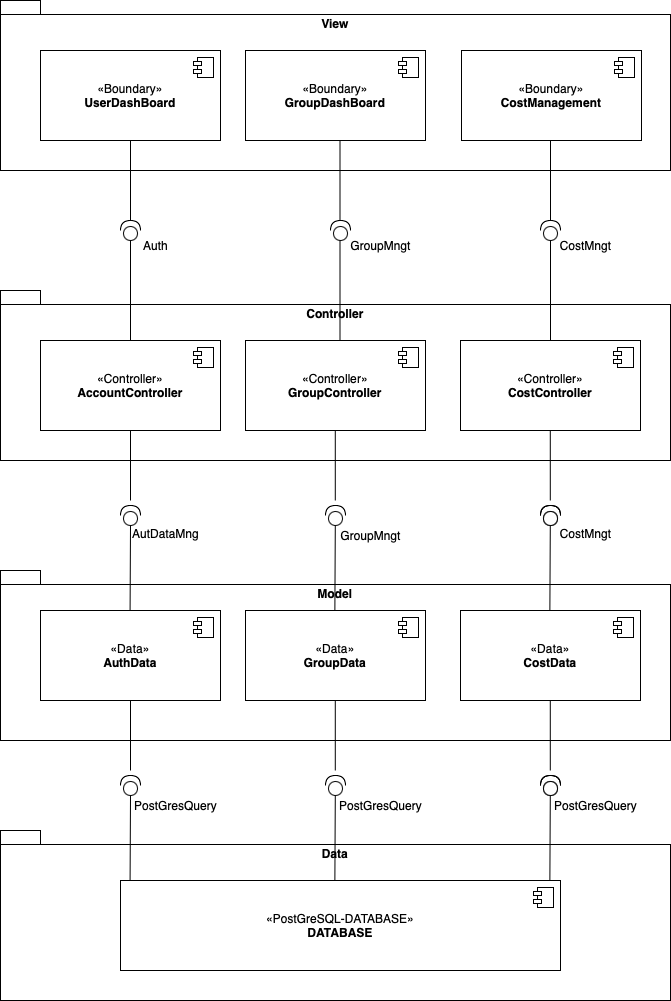
\includegraphics[scale=0.45]{images/ComponentDiagramV1.3.png}
\end{center}

In questa iterazione, aggiorniamo il diagramma dei componenti rispetto all'iterazione 1 data l'introduzione dei costi. 
Partendo dai casi d’uso selezionati per questa iterazione e procedendo con l’utilizzo delle euristiche di design, è stato possibile progettare l’architettura software del sistema \textbf{Spendly}.  

